\newcommand{\sig}{\sigma}
\newcommand{\Sig}{\Sigma}
\newcommand{\eps}{\epsilon}
\newcommand{\del}{\delta}
\newcommand{\ah}{\alpha}
\newcommand{\lam}{\lambda}
\newcommand{\Lam}{\Lambda}
\newcommand{\gam}{\gamma}
\newcommand{\kap}{\kappa}
\newcommand{\rarr}{\rightarrow}
\newcommand{\larr}{\leftarrow}
\newcommand{\Rarr}{\Rightarrow}
\newcommand{\Larr}{\Leftarrow}

\newcommand{\ol}{\overline}
\newcommand{\dagg}{\dagger}
\newcommand{\mbb}{\mathbb}
\newcommand{\contra}{\Rightarrow\Leftarrow}
% for cross product
\newcommand{\lc}{\langle} %<
\newcommand{\rc}{\rangle} %>
% linear alg
\newcommand{\inv}{^{-1}}
\renewcommand{\vec}[1]{\boldsymbol{#1}}
\newcommand{\kth}{^{(k)}}
% order 
\newcommand{\cO}{\mathcal{O}}
% gradient
\newcommand{\grad}{\nabla}
\newcommand{\ddx}{\frac \partial {\partial x}}

%other shortcuts
\newcommand{\ben}{\begin{enumerate}}
\newcommand{\een}{\end{enumerate}}
\newcommand{\beq}{\begin{quote}}
\newcommand{\enq}{\end{quote}}
\newcommand{\hsone}{\hspace*{1cm}}
\newcommand{\hstwo}{\hspace*{2cm}}

\newcommand{\noi}{\noindent}
\parskip 5pt
\parindent 0pt

\documentclass[a4paper]{article}
\usepackage{amsmath,amssymb,algorithmic}
% \usepackage{pdfpages}
\begin{document}
\title{Scientific Computing CS660 Fall '11\\Notes after the midterm}
\author{Angjoo Kanazawa}
\maketitle
\section{Class 13 October 25th 2011}
\label{sec:class13}
\subsection{HW2 answers}
\textbf{Problem 1b}: to compute many $N$, compute $S_N = \phi(x_1) + \cdots +
\phi(x_n)$, take $N$ samples, divide by $N$ will give us $I_N$. THe
error is $E_N = I-I_N$. TO generate $I_{N+1}$, take $S_{N+1} = S_N +
\phi(x_{N+1})$ to compute $I_{N+1}$. But this way $E_{N+1}$ is not
independent from $E_N$. (Left top figure on the answers).

(Doing it entirely independently (how i did it) is the lower figure)
Plotted $\log_N$ vs $\log(\frac{\sig}{\sqrt{N}}$
The observation was that it somewhat follows the bound. 

Our bound, $\frac{\sig}{\sqrt{N}}$, comes from chebychev
$P(|\frac{S_N}{N} - \mu| \ge c) \le \frac{\sig^2}{Nc^2}$.
So if we want this $P$ to be 95\%, then $c\le
\frac{\sig}{\sqrt{0.5N}}$. So loosely speaking, the error $E_N = I-I_N
\approx \frac{\sig}{\sqrt{0.5N}}$. The point of the question was that
it's not exact.

On Page 3 of the solution, there's the definition of histogram for
question 1c.

\textbf{Problem 2}: 
In P1, the error was $E_N = \frac{\sig^2}{\sqrt{N}}$
If the variance is $\sig^2$, std $\sig$, then log of $E_N$ is $\log
\sig - \frac{\log(0.5N)}{2}$. 

In here, we expected the error to be $\frac{\sig^2}{\sqrt{N}}$. If
that were to happen, same derivation would give $\log(E_N)\approx
2\log(\sig) - \frac{\log(0.5N)}{2}$.
The blue line (boundary) would've been $2\log(\sig) -
\frac{\log(N)}{2}$ and $E_N$ will hover around there. But it didn't
work!! Because $sin(\pi X) = sin(\pi(1-X))$, nothing changed. Function
had to be monotone.

\textbf{midterm:}
Equally distributed, 3 topics: floating pt/round off errors, mc,
matrix factorization (big picture). (no newton's method, no machine
representation of numbers)

\subsection{Eigenvalue Hessemberg}
Why do we want to reduce the matrix to Hessemberg form: Because doing
$QR$ on Hessenberg is $\mathcal{O}(n^2)$ instead of
$\mathcal{O}(n^3)$.

How to make a hessemberg matrix:
$A$ is a big full matrix. Now $QA$ will make everything below the
second entry of first column to 0. You can do that with Householder
transformation, or givens rotation. 

However we do this, $QAQ^T$ will not mess up the 0s.
\begin{align*}
 QAQ^T &= [Q(QA)^T]^T\\
\end{align*}
Applying to $Q$ to $(QA)^T$ will leave the first row alone, so
$[Q(QA)^T]^T$ still keeps the first column's entry below 2 to 0.

Exercise, go back, do: can we perform $QAQ^T$ where $Q$ is a
householder transformation s.t. $QAQ^T$ is a first step hessemberg
matrix. The reason why this works is because householder is in the
$n-1$ subblock, so it doesn't do anything row 1. (It's like the 2nd
household transformation in the QR reduction)


$QR$ iteration for the eigenvalue problem:
\begin{enumerate}
\item[0] Reduce $A$ to hessenberg form, formally, $PAP^T = H$, where $P$
  orthogonal. (do $n-1$ householder transformation $P_2$).$A_0 = H$
\item[1-k] Iterate, $A_K = Q_KR_K$, $A_{K+1} = R_KQ_K$
\end{enumerate}
Doing this $A=QR$ is $\mathcal{O}(n^3)$, but to do this until
conversion (see $\eps$ in below diagonal, is $n$, so total
$\mathcal{O}(n^4)$ (without making $A$ into upper hessenberg).
If $A$ wer hessenberg, doing $QR$ is $\mathcal{O}(n^2)$ instead of
$\mathcal{O}(n^3)$, so the total cost is $\mathcal{O}(n^3) +
\mathcal{O}(nn^2) = \mathcal{O}(n^3)$ with hessemberg.

\pagebreak

\section{Class 14 November 1st}
\label{sec:class14}
Midterm: median 22, mean 20.8, max:29

\subsection{Midterm}

\textbf{Problem 1}:
Given $Ax=b$, $A\hat x = b + \delta b$: $A(x-\hat x) = b -b \delta b$
so 
\begin{align*}
x-\hat x &= A^{-1}(\delta b)\\
||x-\hat x|| &\le ||A^{-1}||||\delta b||\\
\end{align*}
And
\begin{align*}
  b&=Ax\\
||b|| &\le ||A|| ||x||\\
\frac{1}{||x||} &\le \frac{||A||}{||b||}\\
\end{align*}
So
$$
\frac{||x-\hat x||}{||x||} \le ||A|| ||A^{-1}|| \frac{||\delta b||}{||b||}
$$
\noi
\textbf{Problem 2}: 
\begin{enumerate}
\item[a] QR factorization by gram-schimid
\item[b] Making $r_{ik} = <\hat q_k, q_i>$ from $r_{ik} =<a_k, q_i>$,
  doesn't change anything. Because
  \begin{align*}
    r_{23} = \lc\hat q_3, q_2\rc \\
&= \lc a_3 - r_{13}, q_2\rc\\
&= \lc a_3, q_2 \rc - r_{13}\lc q_1, q_2 \rc
\end{align*}
\item[c] Real question is: Will $q_3$ be orthogonal to $q_2$ and
  $q_1$? Look at $\hat q_3$ after $i$th loop is done. $\hat q_3 = \lc
  a_3 - r_{13}q_1 - r_{23}q_2, q2 \rc = \lc a_3, q_2\rc - r_{13}\lc
  q_1, q_2\rc = -r_{23}\lc q_2, q_2 \rc$
Problem is $\lc q_1, q_2\rc$ could be non-zero because of round-off
error.
But if we did the second way, $\lc \hat q_3, q_2 \rc = \lc a_3 - r_{13}q_1, q_2 \rc -
r_{23}\lc q_3, q_2 \rc$, is a little bit less-sensitive to round-off
errors. Called the modified-Gram Schmid. (This can't be run parallel)
\end{enumerate}

\subsection{Singular Value Decomposition}
\label{sec:SVD}

Let $A\in \mathbf{R}^{m\times n}$. $A$ can be factored as $$A=U\Sigma
V^T$$, $U$ is $m$ by $m$, sigma is $m$ by $n$, a diagonal matrix, where
the entries are $sig_1, \dots, sig_n$, everywhere else 0. $sig_i$'s
are called the singular values, and $\sig_1 \le sig_2 \le \cdots \le
\sig_n \le 0$.
$V^T$ is $n$ by $n$. Where $U^TU = I_m$ and $V^TV = I_n$.

How to use:
\textbf{Least Squares}: minimize $||b-Ax||_2$, find $x$. 
  \begin{align*}
    ||b-Ax||_2^2 &= \lc b-Ax, b-Ax \rc \\
&= \lc b-U\Sigma V^Tx, b-U\Sigma V^Tx \rc \\
&\text{ let $\hat x = V^Tx$}\\
&= \lc U(U^Tb-\Sigma\hat x), U(U^Tb-\Sigma\hat x) \rc \\
&= \lc U^TU(U^Tb-\Sigma\hat x), U^TU(U^Tb-\Sigma\hat x) \rc \\
&= \lc U^Tb-\Sigma\hat x, U^Tb-\Sigma\hat x \rc \\
&\text{ let $\hat b = U^Tb$}\\
&= \lc \hat b-\Sigma\hat x,  \hat b-\Sigma\hat x \rc \\
&= || \hat b - \Sigma \hat x ||^2_2
  \end{align*}
This is $$
\begin{pmatrix}
 \hat b_1 \\ \hat b_2 \\ \vdots \\ \hat b_m
\end{pmatrix}
-
\begin{pmatrix}
 \sig_1 \hat x_1 \\ \vdots \\ \sig_n\hat x_n \\ 0 \\ \vdots 0
\end{pmatrix}
$$
So to minimize, set $\sig_k\hat x_k = \hat b_k$, or $$\hat x_k =
\frac{\hat b_k}{\sig_k}$$

The norm of minimum norm solution is $\sqrt{\hat b^2_{n+1} + \cdots +
  \hat b_m^2}$, provided $\sig_n > 0$. If all $\sig_j > 0$, then $\hat
x, x$ are unique. aka $A$ is of full rank. If some of them are zero,
then $\exists$ multiple solutions $\hat x$ and $x$. Rank of $A$ is the
index of smallest nonzero $\sig_j$s.

To solve this problem, compute $U, V$ and $\Sigma$, fing $\hat b$,
find $\hat x$, find $x=V\hat x$.

\textbf{Remember}: least squares solution can be found from $A^TAx =
A^Tb$:
\begin{align*}
  A^TAx &=A^Tb\\
V\Sigma^TU^T U\Sigma V^T x &= V \Sigma^T U^Tb\\
V[\Sig_1 0][\Sig_1; 0]V^T x&= V \Sigma^T U^Tb\\
V\Sig_1^2 V^T x &= V[Sig_1 0][U^Tb]\\
\Sig_1^2 V^Tx &=\Sig_1[U^Tb]\\
\end{align*}
This is just like the one before where $V^Tx = \hat x$,
$\hat b = U^Tb$.

\subsection{Pseudo-inverse}
Of a rectangular matrix $A$, is written:
$$A^\dagger = (A^TA)^{-1}A^T$$
$(A^TA)^{-1}$ is square times wide rectangle, so a wide rectangle. 
Property: $A^\dag A = (A^TA)^{-1}A^A = I$.

Given $A = U\Sig V^T$, 
\begin{align*}
  A &= U\Sig V^T\\
A^TA &= V\Sig_1^2 V^T\\
(A^TA)^{-1} &= (V\Sig_1^2 V^T)^{-1} = (V^T)^{-1}(\Sig_1^2)^{-1}V^{-1}\\
&=V\Sig_1^{-2}V^T\\
\end{align*}
So 
\begin{align*}
A^\dagger = (A^TA)^{-1}A^T &= V\Sig_1^2 V^T V([\Sig_1 0]) V^T\\  
&=V([\Sig_1^{-1} 0])U^T
\end{align*}

\section{Class 16 November 3rd 2011}
\label{sec:class16}

\subsection{Continue on SVD}
\label{sec:svd2}

Given $A\in \mathbf{R}^{m\times n}$, $m>n$, $A=U\Sig V^T$, $A$ full
rank.
$A = [U_1 U_2][\Sig_1 ; 0] V^T$ wher $U_1$ is m by n, $U_2$ is m by
$m-n$.
And
\begin{align*}
  U^TU &= [U_1^T; U_2^T][U_1 U_2]\\
&=
\begin{pmatrix}
U_1TU_1  & U_1^TU_2\\
U_2^TU_1 & U_2^TU_2
\end{pmatrix}
&=I =
\begin{pmatrix}
  I & 0 \\ 0 & I
\end{pmatrix}
\end{align*}
Because $U_1^TU_1 = I_n, U_2^TU_2 = I_{m-n}$, and $U_1^TU_2=0$

$A^T = V[\Sig_1 0][U_1^T; U_2^T] = V\Sig_1U_1^T$.
Consider $w\in \mathbf{R}^m$, look at $A^Tw = V\Sig_1U_1^Tw$. If $w\in
range(U_2)$, $w = U_2z$ for some $z$, so
$$A^Tw = V\Sig_1U_1^TU_2z = 0$$
i.e. $range(U_2) \subseteq null(A^T)$, $\supseteq$ is also true.
So $$null(A^T) = range(U_2).$$

\textbf{Pf}[$range(U_2) \supseteq null(A^T)$]
Suppose $w \in null(A^T)$, i.e. $A^Tw = 0$. 
$w = U_z$, for some $z$
\begin{align*}
  w &= U_z\\
&= U_1z_1 + U_2z_2
A^Tw &= V\Sig_1 U_1^T (U_1z_1+U_2z_2)
&=V\Sig_1 z_1 + 0
\end{align*}
If $z_1 \neq 0 \Rarr \Sig_1z_1 \neq 0$ $\contra$ because the
assumption $range(U_2)\subseteq null(A^T)$, $A^Tw$ should be 0. So it
has to be that $z_1 = 0$.  $\therefore w \in range(U_2)$

Another point:
COlumns of $U_1$ span the range of $A$. Range of $A:=\{Av | v\in
\mathbf{R}^n\}$.
Given $Av = U_1(\Sig_1 V^Tv)\subseteq range(U_1)$

We can see that $range(A)$ and $null(A^T)$ are orthogonal to each
other. (This is a known fact in linear algebra, but SVD makes it intuitive)

end of matrix factorization!
\section{New topic:Optimization}
Given $f: \mathbf{R}^n \rarr \mathbf{R}$, we want to find $x\in
\mathbf{R}^n s.t. f(x)$ is minimal (i.e. $-f(x)$ is maximal).
We may want to find:
\begin{itemize}
\item Global minimum $\hat x s.t. f(\hat x) le f(x) \forall x$
\item Local  minimum $\hat x s.t. f(\hat x) le f(x) \forall x$ near $\hat x$
  (rigorously: near means in some radius $r$.).
\end{itemize}
In this class we're looking for a local minimum.

If $x$ is a local minimum value, consider $\phi(\ah) = f(x+\ah d) $, where $d\in
\mathbf{R}^n$, some other vector, $\ah \in \mathbf{R}$.
Now look $\phi(\ah)$'s taylor series: $  \phi(0) + \phi'(0)\ah + \cO(\ah^2)$
\begin{align*}
\phi'(\ah) &= [\grad f(x+\ah d)]^Td\\
\phi'(0) &= [\grad f(x+\ah d)]^Td\\
\end{align*}
(Where $\grad f =
\begin{pmatrix}
  \frac{\partial f}{\partial x_1} &\vdots &  \frac{\partial f}{\partial x_n}
\end{pmatrix}$)

Suppose $\grad f(x) \neq 0$. \emph{Claim}: $\exists d s.t. [\grad
f]^Td < 0$.
Does such $d$ exist? yes, take $d = -\grad f(x)$. There's at least
one.

For any such $d$, $\phi(x+\ah d) = \phi(x) + [(\grad f(x))^Td]\ah + \cO(\ah^2)$
$\phi(x)$ is $f(x)$, and $(\grad f(x))^Td < 0$

When $\ah \ll$, positive, $\cO(\ah^2)$ is negligible incomparison to
$[(\grad f(x))^Td]\ah$. So $\phi(x+\ah d) < f(x) \forall$ small
positive $\ah$. 
$\contra$ because we started off with a local minimum! $\Rarr \grad
f(x) = 0$.

Summary: A necessary condition for $x$ to be a minimizer is that
$\grad f(x) = 0$. (not sufficient): called the 1st order necessary condition.
This can be solved by doing newton's method on $F=\grad f(x)$.

Check the second derivative, if concave (second derivative positive), then we have a local minima.

Look at 3-term taylor series.
$\phi''(\ah) = d^T\grad^2f(x+\ah d)d$, where $\grad^2f(x+\ah
d)$ is a matrix with $(i,j)$ entry given by $H = \frac{\partial^2
  f}{\partial x_i \partial x_j}(x+\ah d)$. This is the
\textbf{Hessian} matrix.
So $\phi''(0) = d^T\grad^2 f(x) d = d^THd$
So:
\begin{align*}
\phi(\ah) &= f(x+\ah d) = \phi(0) + \phi'(0)\ah + \frac{1}{2}\phi''(0)\ah^2 +
\cO(\ah^3)\\
&= f(x) + [\grad f(x)]^Td]\ah + \frac{1}{2}d^THd \ah^2 + \cO(\ah^3)
(\text{ because $x$ is a local minimum, } \grad f(x)]^Td == 0, \text{
  and } d^THd < 0 \forall d)\\  
\end{align*}

(if $d^THd < 0$, then $f(x+\ah d) < f(x)\forall \ah \ll$ ( $\contra$ just
like the other reasoning)).

So another necessary conditions is $H = \grad^2f(x)$ has to be positive
semidefinite, this is calloed the 2nd order necessary condition.

Note that these together are not sufficient.

\emph{Example:} $n=2$, $f(x) = \frac{1}{2}x_1^2 + x_1 + x_2^3$
then $\grad f =
\begin{smallmatrix}
x_1+1 & 3x_2^2  
\end{smallmatrix} = \begin{smallmatrix}
0 & 0
\end{smallmatrix}$ set $x_1 = -1, x_2 = 0$.
So $\grad^2 f =
\begin{smallmatrix}
  1 & 0 \\ 0 & 6x_2
\end{smallmatrix} =
\begin{smallmatrix}
  1 & 0 \\ 0 & 0
\end{smallmatrix}$ at $x=(-1,0)$

Condition for a matrix to be positive definite is that all its
eigenvalues are strictly positive. Semi-definite is all its
eigenvalues are $le 0$. So this is $H$ that satisfies the condition
and we have two necessary conditions satisfied at $x=(-1, 0)$.
But it's not because we can find a point $\tilde x=(-1, x_2)$
$f(\tilde x) = \frac{1}{2} + x_2^3 < f(x) = -\frac{1}{2} \forall x_2
le 0$.

\textbf{Sufficient conditions}:
\begin{enumerate}
\item $\grad f(x) = 0$
\item $\grad^2 f(x) = H$ is positive-definite. (i.e. in 2-D function
  is concave at this point)
\end{enumerate}

If we have some $x$ not a minimizer, algorithm will chose a $d$
s.t. $f(x+\ah d) < f(x)$. One condition for $d = -\grad f(x)$.

Another approach: try to find a root of the equation $F(x) = \grad
f(x) = 0$.

Recall \emph{Newton's method}: In 1-D, $x_{n+1} = x_{n} +
\frac{-f(x_n)}{f'(x_n)}$.
In N-D, it's $J_F(x_n)d = -F(x_n)$ (not the same $d$)

\pagebreak
\section{Class 17,18 November 15th 2011} Missed for grace hopper 
% 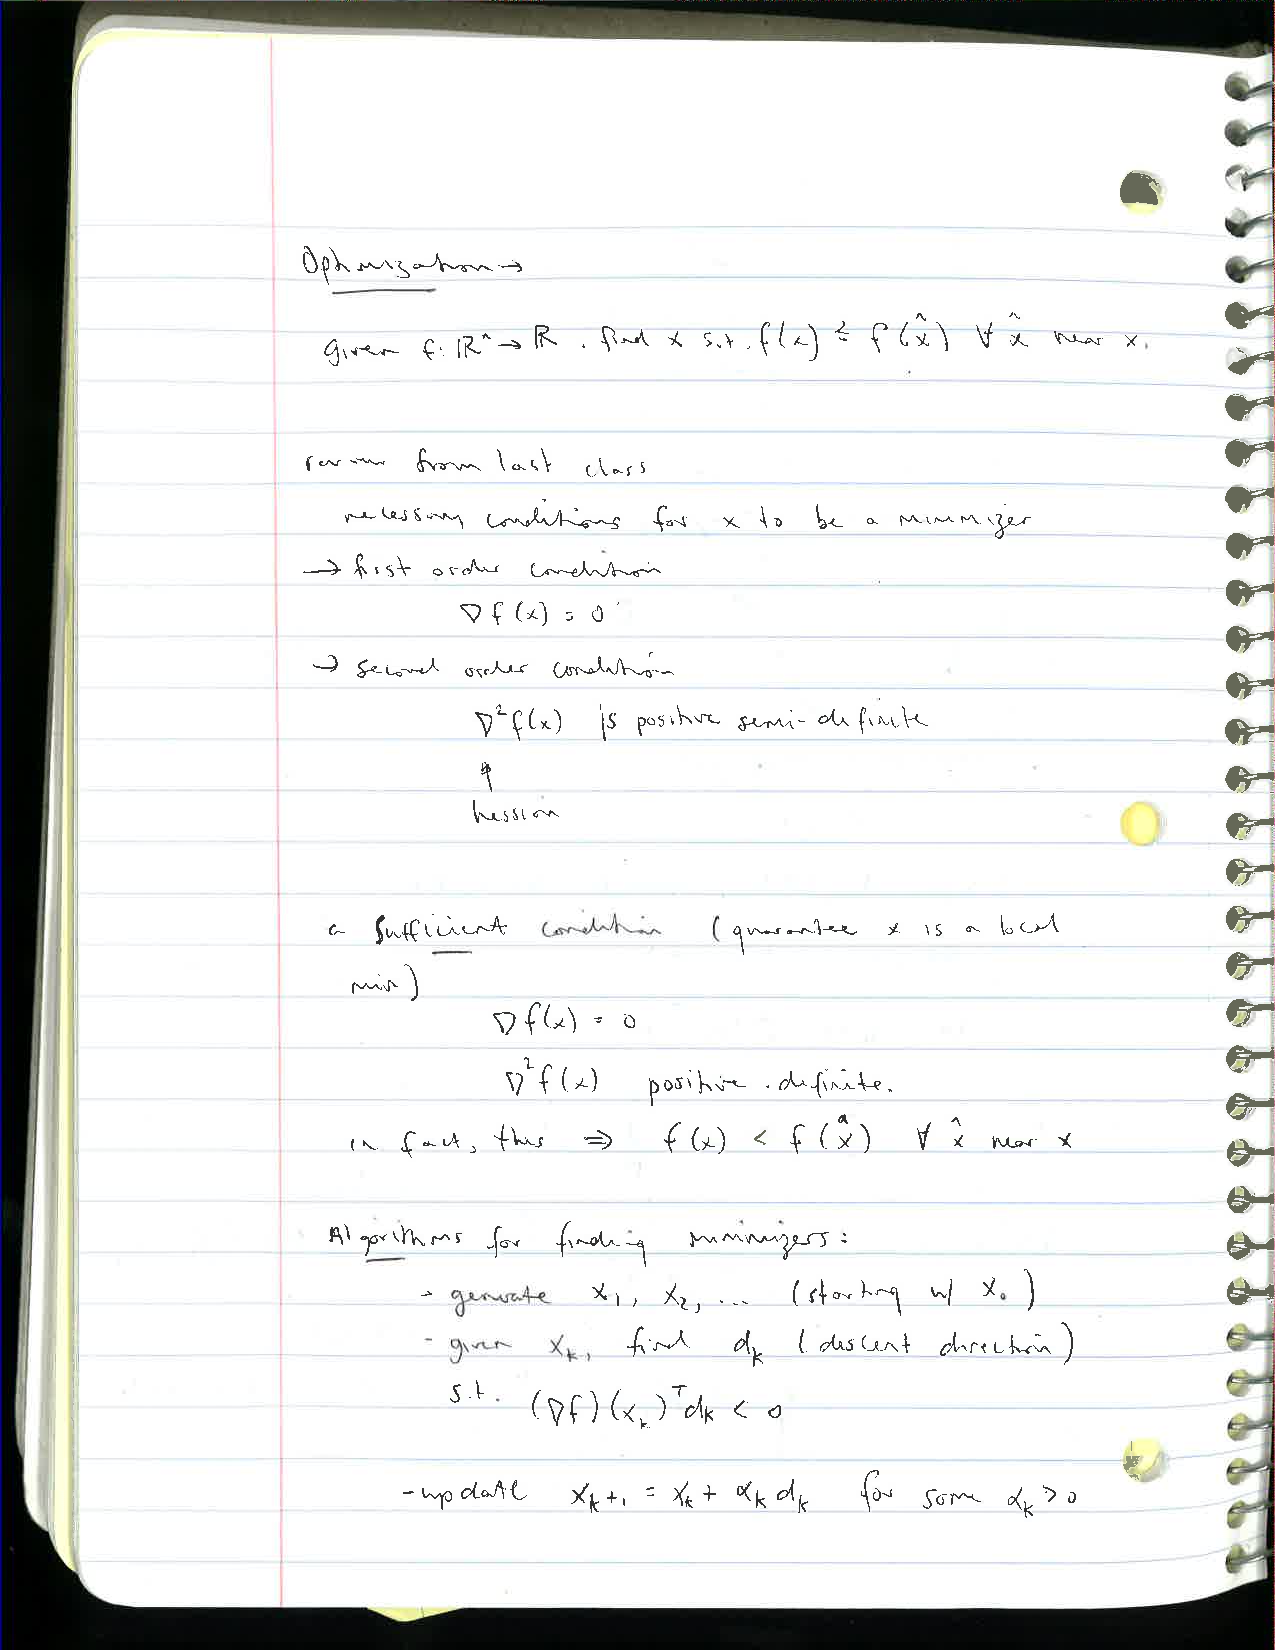
\includepdf[pages={-}]{jessyNote1.pdf}
\section{Class 19 November 15th 2011}
% 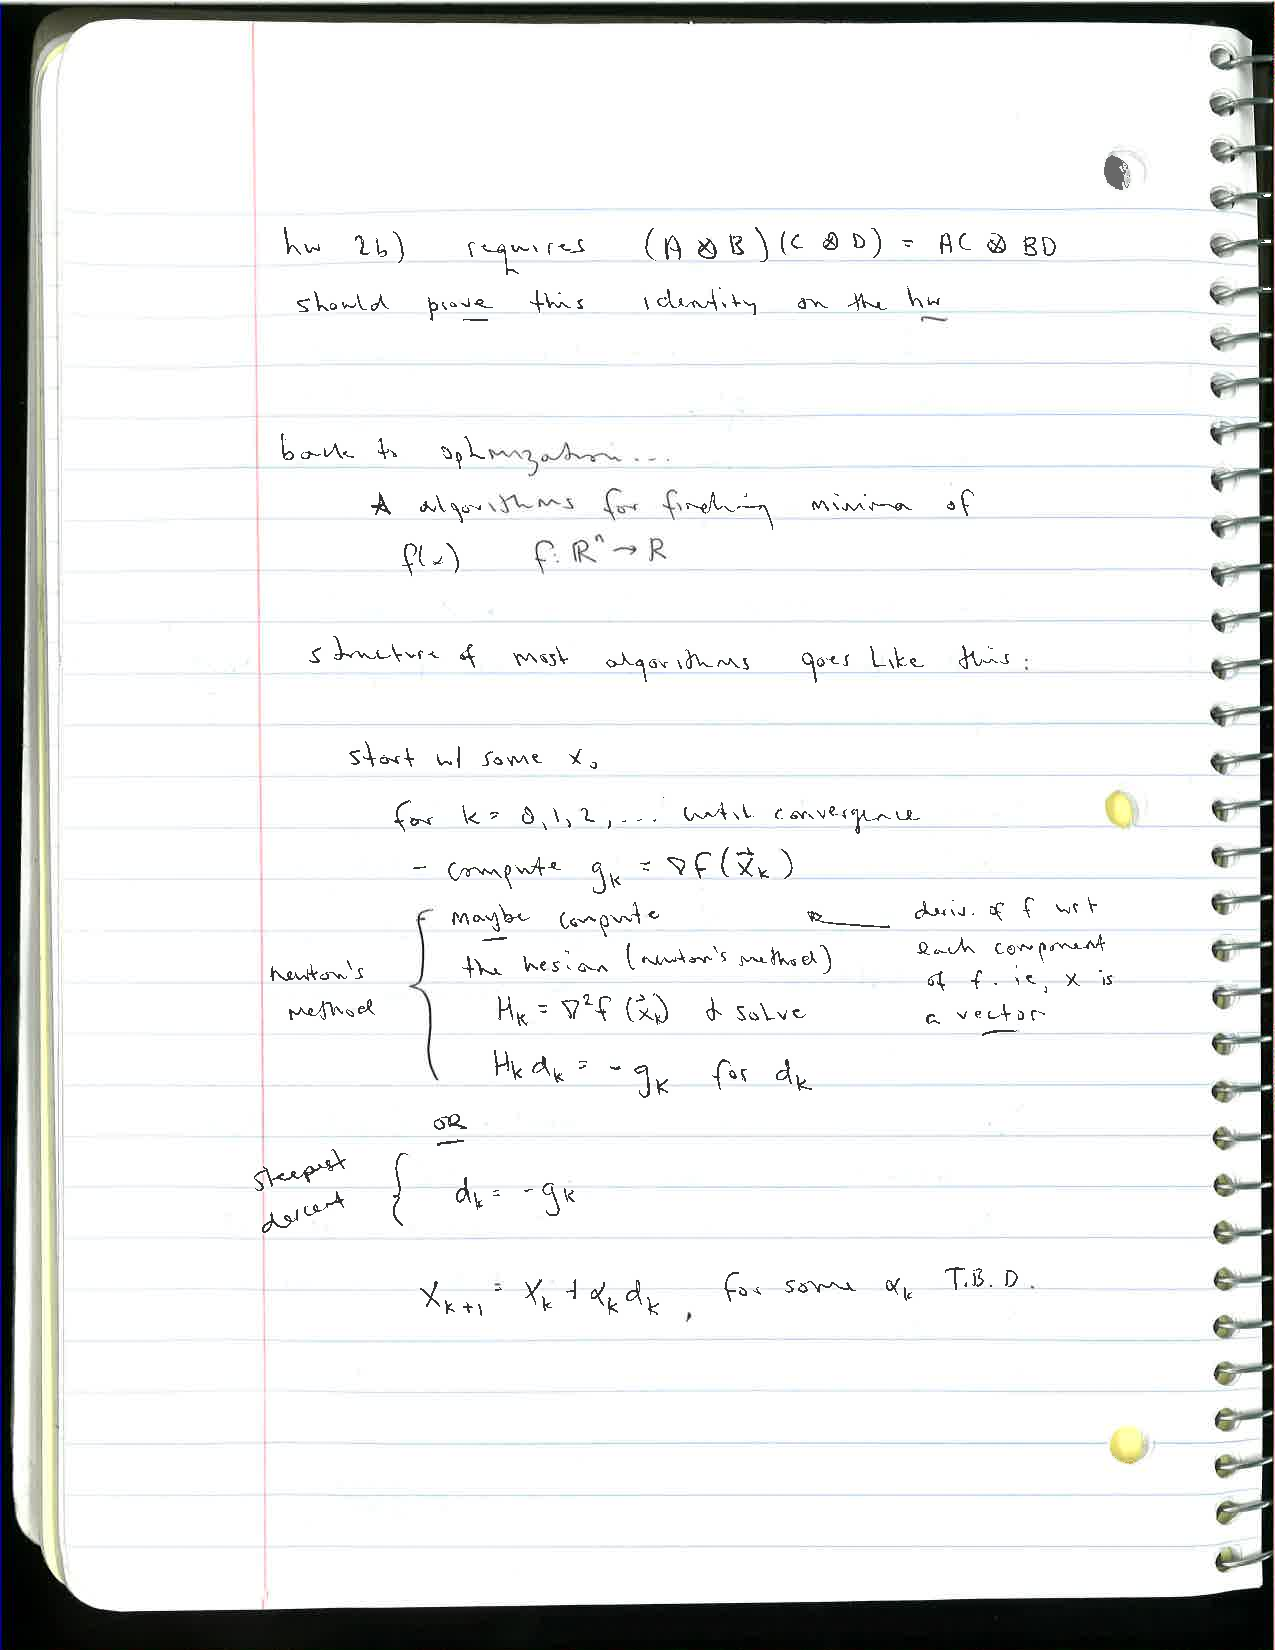
\includepdf[pages={-}]{jessyNote2.pdf}
\label{sec:class19}

\subsection{Optimization}
$f:\mathbf{R}^n \rarr \mathbf{R}$ Iteration $x_{k+1} \larr x_k +\ah_k
d_k$, where $d_k$ is the descent direction $d_k^Tg_k < 0$, and $\ah_k$
is the step length obtained from line search.

From last time: Choose $\ah_k$ s.t. $$f(x_k+\ah_kd_k) \le f(x_k) + \mu
\ah_kd_k^Tg_k$$ where $\mu$ is a fixed parameter. Called the \emph{Armijo condition}.
Refer to the graph on the notebook, but $\phi(\ah) = f(x_k+\ah d_k)$,
$\phi(0) = f(x_k)$, $\phi'(0) = \grad f (x_k)^Td_k = d_k^Tg_k$, and
$\phi_\mu(\ah) = f(x_k) + \mu\ah d_k^Tg_k$.

Another way to do line search: try to find $\ah$ near the value that
minimizes $\phi(\ah)$.
Where $\phi'(\ah) = [\grad f (x_k+\ah d_k)]^Td_k$, such minimizer of $\phi$ (if it
exists) satisfies $\phi'(\ah) = 0$.

Strategy: Choose $\ah_k$s.t. $\phi'(\ah)$ is not too large. That is,
require $$|\phi'(\ah)| \le \eta |\phi'(0)|$$ for some fixed constant
$\eta$ (example $\eta = .9$).

Guess $\ah$ by evaluating $|\grad f (x_k+\ah d_k)]^Td_k|$ compare it
to $|g_k^Td_k|$. Called the \emph{Wolfe Condition}.
This way is more expenisve, because we need to compute the $\grad f$,
which involves $n$ computations, as opposed to computing $f$ is just
single real value. 
But this is prefered because: we are requiring the derivative to be
smaller, it force us to chose a bigger step sizes and move closer to
the minimum sooner. (Because say we have a candidate $a$ very close to
$0$, the slope of $\phi'(a)$ will be very close to $\phi(0)$, so it
will prevent us from chosing $\ah$ that's too close to 0.

So far we've seen
\begin{itemize}
\item steepest descent $d_k = -g_k$ (slow but cheaper)
\item Newton's method $d_k$ solves $H_kd_k = -g_k$, called the
  Hessian. $\grad^2 f(x_k)$ is the descent direction iff $H_k$ is
  positive-definite. ($d_k^Tg_k < 0 \rarr -g_k^TH_kg_k$ is guaranteed to be $< 0$ if $H_K$
positive-definite, but may happen by luck so we want the condition
example: $g_k=[1,0], H_k=(\begin{smallmatrix}  1 & 0 \\ 0 & -1 \end{smallmatrix})$).

Evaluating the hessian and solving system is very expensive.
\end{itemize}

\subsection{Quasi-Newton Methosd}
\label{sec:quasi-newton}

This method will construct $B_K$, an approximation to $H_k$ somehow.
Algorithm:
\begin{algorithmic}
  \STATE{ Start with an arbitrary $x_0$, $B_0$ ($=I$, for example), $g_0 = \grad f(x_0)$}
  \FOR{ $k=0,1,2,\dots$ until convergence}
    \STATE{solve $B_kd_k = -g_k$}
    \STATE{update $x_{k+1} = x_k + \ah_kd_k$}
    \STATE{compute $g_{k+1} = \grad f(x_{k+1})$}
    \STATE{update $B_{k+1} = B_k - $ (some update)}
  \ENDFOR
\end{algorithmic}
Q: How to choose $B_{k+1}$??

One approach: Consider $H(x_k)$ when $f$ is a quadratic
function. $$f(x) = \frac{1}{2}x^TQx + b^Tx + c$$, a typical quadratic
function.
$\grad f(x) = Qx+b$ (exercise)
$\grad f(x+d) = Qx + Qd + b$, and $\grad f(x+d) - \grad f(x) = Qd$.
ALso, $\grad^2 f = Q$. This implies that $$Hd = \grad^2f d = Qd = g(x+d) - g(x)$$ We
will try to mimic this relationship for general $f$. 

Try to eforce this conversation as follows:
Choose $B_{k+1}$ to satisfy $B_{k+1}d_k = g_{k+1} - g_k$. But this is
not enough to get a good estimate so in addition,
$B_{k+1}v = B_kv$ $\forall v$ orthogonal to $d_k$ (because the first
condition is just 1-D, this make sure that we don't do anything to
whatever that's not in the same direction).

Consider
$$B_{k+1} = B_k - \frac{(B_kd_k - (g_{k+1} - g_k))d_k^T}{d_k^Td_k}$$
Check: 
\begin{align*}
B_{k+1}d_k &= B_kd_k - \frac{(B_kd_k - (g_{k+1} -
  g_k))d_k^Td_k}{d_k^Td_k}\\  
&= B_kd_k - (B_kd_k - (g_{k+1} - g_k))\\  
&= g_{k+1} - g_k
\end{align*}
Also 
\begin{align*}
  B_{k+1}v &= B_kv - \frac{(B_kd_k - (g_{k+1} -
    g_k))d_k^Tv}{d_k^Tv}\\  
&= B_kv - 0 \text{ for $v \perp d_k$}
\end{align*}
This is called the \emph{Broyden's method}, a rank-1 update. Way
cheaper than evaluating the hessian.

If $H$ is a hessian, it would be a symmetrix matrix (it's a second
derivative $\frac{\partial^2 f}{\partial x_i\partial x_j}$). But $B_k$
by Broyden's method is not symmetric.

So \emph{Symmetric variant:}
Let $y_k = g_{k+1} - g_k$, $$B_{k+1} = B_K +
\frac{(y_k-B_kd_k)(y_k-B_kd_k)^T}{(y_k-B_kd_k)^Td_k}$$

\pagebreak

\section{Class 20 November 17th 2011}
\label{sec:class20}
Review of the HW3 \#2:
$\hat A_c = A_c + E$, we want $A$. THere is a linear relation between
$A$ and $A_c$. Unravel $A,A_c,\hat A_c$ column wise to get $a,a_c,\hat
a_c$.
The naive computation was to solve $Ka = \hat a_c$ but this runs out
of memory, or takes way too long.

$K$ has the form $B \otimes C$. Question was how do you take advantage
of this and solve $Ka = \hat a_c$.  Supposed we wanted to solve $(B
\otimes C)x = y$
$B \otimes C =
\begin{pmatrix}
  b_{11}C & b_{12}C & \cdots & b_{1n}C\\
  \vdots &  & \cdots & \vdots \\
  b_{11}C & b_{12}C & \cdots & b_{1n}C\\
\end{pmatrix}
$
Change $x$ s.t. it's $m$ by $n$.
THen, the first block is
\begin{align*}
C(b_{11}x_1 + b_{12}x_2 + \cdots + b_{1n}x_m)  &=C[x_1 , x_2, \cdots, x_m]
\begin{pmatrix}
  b_{11} \\ b_{12} \\ \vdots \\ b_{1n}
\end{pmatrix}
&= \text{ transpose of 1st row of $B$ is 1st col of $B^T$}
\end{align*}
So
$$CXB^T=Y$$ where $X$ and $Y$ are reshaped versions of $x$ and $y$ in
blocks.
So the solution is $X=C\inv Y B^{-T}$. Let $C= U_c\Sig_cV_c^T$ and
$B=U_b\Sig_bV_b^T$, then $X$ is $V_c\Sig_c\inv U_c^TY(U_b\Sig_b\inv V_b^T)$

\subsection{Quasi-Newton Methods}
\label{sec:quasi-newton}
From before:
\begin{algorithmic}
  \STATE{ Start with $x_0$, $B_0$ ($=I$, for example), $g_0 = \grad f(x_0)$}
  \FOR{ $k=0,1,2,\dots$ until convergence}
    \STATE{solve $B_kd_k = -g_k$}
    \STATE{update $x_{k+1} = x_k + \ah_kd_k$}
    \STATE{compute $g_{k+1} = \grad f(x_{k+1})$}
    \STATE{update $B_{k+1} = B_k - $ (some update)}
  \ENDFOR
\end{algorithmic}
 We looked at \emph{Broyden's method} $$B_{k+1} = B_k - \frac{(B_kd_k
   - (g_{k+1} - g_k))d_k^T}{d_k^Td_k}$$
That satisfies both conditions, but $B_k$ may not be symmetric (and
should be because $H_k$ is).

Symmetric variant: Let $y_k = g_{k+1} - g_k$, $$B_{k+1} = B_K +
\frac{(y_k-B_kd_k)(y_k-B_kd_k)^T}{(y_k-B_kd_k)^Td_k}$$
We can't impose the second condition that $B_kv = 0$ for $v\perp d_k$.
Also $B_k$ may not be positive definite.

\emph{Further refinment}: $$B_{k+1} = B_k -
\frac{(B_kd_k)(B_kd_k)^T}{d_k^TB_kd_k} + \frac{y_ky_k^T}{y_k^Td_k}$$
It's easy to verify that $B_{k+1}d_k = g_{k+1} - g_k$

\textbf{Theorem} If $y^Td_k > 0$ then $B_{k+1}$ is positive definite.

 $y^Td_k>0$ means $g_{k+1}^Td_k > g_k^Td_k$. $d_k$ taht we're working
 with is a descent direction, so both sides of the inequality is
 negative, so it means the next descent direction is not as negative as
 the one before. i.e. $$-g_k^Td_k > -g_{k+1}^Td_k$$

Returning to Wolfe condition for line search, it says $|g_{k+1}^Td_k |<
\eta |g_k^Td_k|$ for some $\eta < 0$.

This is equivalent to

$$-g_{k+1}^Td_k \le |g_{k+1}^Td_k| < \frac{1}{\eta}|g_{k+1}^Td_k| \le
-g_k^Td_k$$
(given $\eta < 1$). The end equality is the same condition about the theorem. i.e. if we
impose the Wolfe condition, $B_{k+1}$ is positive definite.
This refined version where it guarantees positive definite ness is
called the \textbf{$BFGS$ method}.

\subsection{Constrained Optimization}
\label{sec:constrainedoptimization}

Now we want to $ \min f(x)$ $f\in \mathbf{R}^n$ subject to $g(x)
\le 0$, where $g: \mathbf{R}^n \mapsto \mathbf{R}^m$.

ex. $n=2$. $x_2 = x_1+1$, $g(x) = x_2 - x_1 - 1 \ge 0$, then the
possible region is the parts above the line. 

Find $x$ in constraint set that minimizes $f$.
\pagebreak
\section{Class 22 (skipped one) Nov 29th}
HW3: first part, to show the error is proportional to $\kap(Q)$,
taylor series approximation is involved. Number of steps is
approximately $\kap(Q)$ based on the taylor approximation, assuming
that $\kap(Q)$ is big. Part b of problem 2, enforce certain
equalities, gradually tweak so taht the equality is true. Do line
search in several different ways and he talked about a way in class to
do tweaking, do that for number 2. For number iii, use matlab
minimization function. For i, you might have to do global search, but
tweaking is what he has in mind..

\subsection{Constrained Minimization}

Minimize for $x\in \mathbf{R}$, $f(x)$ subject to $Ax=b$. $A$ is a
full rank $m$ by $n$ wide matrix ($m<n$).
\begin{itemize}
\item Method 1: start with a feasible $\bar x$ (satisfies $A\bar x =
  b$), let $Z=$matrix whose columns span the null space of $A$, $Z\in
  \mathbf{R}^{n\times (n-m)}$. (SVD's
  last $m-n$ columns of V). We can solve this problem by solving $\min
  v\in \mathbf{R}^{n-m}\hat f(v)$, $\hat f(v) = f(\bar x + Zv)$
  (compute the gradient of $\grad_v\hat f=Z^T(\grad_xf(\bar x + Zv))$,
  $grad_v^2 \hat f = H = Z^T(\grad_x^2f(\bar x + Zv))Z$
  then use steepest descent or newton using H)
\item Method 2: Using the first order conditions for minimizing $\hat
  f$, we are led to the equation of the form $\grad f(x)+A^T\lam = 0$
  and $Ax=b$. We want to find $x, \lam$ that satisfies these
  equations. (the first equation says that the gradient is in the
  range space of A) We don't need $Z$ for this method: if $n$ is
  large, computing $Z$ is expensive. 
  
  This is a nonlinear system of equations, to do it we'll discuss it
  in class.
\end{itemize}

For method 1, how do we get $\bar x$, a feasible point?
Suppose we obtained $Z$ by $QR$ factorization. $A^T=QR= [Q_1 Q_2][R_1;
0] = Q_1R_1$, where $Z=Q_2$ $Q_1$ spans the range space of $A$ and
$Q_2$ is the orthogonal complement of $Q_1$ so it spans the null space
of $A$. And $A=R_1^TQ_1^T$. We want $A\bar x = b$:
\begin{align*} 
  A\bar x &= b\\
R_1^TQ_1^T \bar x &=b\\
Q_1^T \bar x = R_1^{-T}b \text{ let }R_1^{-T}b = \hat b\\
&\text{ Define }\hat x = Q_1\hat b\\
Q_1^T\bar x &=  Q_1^TQ_1 \hat b\\
Q_1^T\bar x &=  Q_1^TQ_1 R_1^{-T}b\\
R_1^TQ_1^T\bar x &=  R_1^TR_1^{-T}b\\
A\bar x &=  b
\end{align*}
Now we have $\bar x$.

\subsection{Nonlinear constraint problem }
minimize $f(x)$ for $x\in \mathbf{R}^n$, subject to $g(x)\ge 0$, where
$g:\mathbf{R}^n \mapsto \mathbf{R}^m$. Example: $g(x) = Ax-b$, or
$g_1(x), \dots, g_m(x)$ all $\ge 0$.
Harder problem.
Highlevel statemetn: Minimize the function inside, move closer to the
boundary and see if that changes things.

\textbf{Strategy}:
\begin{itemize}
\item Define $\phi(x)$ s.t. $\phi(x)\rarr \infty$ as $g(x) \rarr 0$.
  \begin{itemize}
  \item \emph{Example}: $\phi(x) - \sum_1^m \log q_i(x)$ means $\log$ is
  well defined, if all $g_i$s approach 0, $\sum_1^m \log q_i(x)\rarr
  -\infty$, so $\phi(x) \rarr \infty$.
\item \emph{Example}: $\phi(x) = \sum_{i=1}^m \frac{1}{g_i(x)^2}$
  \end{itemize}
\item Introduce a scalar parameter $\mu>0$ and consider the function
  $$\hat f_\mu(x)=f(x) + \mu \phi(x)$$ (function of n+1 param, but think of $\mu$ as fixed here)
\item Consider the unconstraint problem $\min_x \hat f_\mu(x)$. As
$x$ approaches the boundary of the constraint set i.e. $g(x)\equiv 0$,
$\mu\phi(x)\rarr \infty$, so the solution/minimizer to this problem will be in
the interior of our constraint, that is $g(x)>0$. This minimizer $x$
depends on $\mu$. i.e. $x=\mu(x)$.
\item next step, is to reduce $\mu$ and do it again.

\end{itemize}
\emph{Claim}: as $\mu\rarr 0$, $x(\mu)\rarr x^*$, the solution to the
constraint problem.

\textbf{Algorithm - the Barrier Method}: For a sequence $\mu_1 > \mu_2 > \dots$, find $x(\mu_i)$, use
$x(\mu_i)$ as the initial value for the problem with parameter
$\mu_i+1$ ($\hat f_\mu(x)$). As $\mu\rarr 0$, the conditioning of the hessian of $\hat
f_\mu(x)$ grows. Meaning makes it harder for newton's method to solve.

\subsection{Nonlinear equations}
$F:\mathbf{R}^n \mapsto \mathbf{R}^n$, where $F=
\begin{pmatrix}
f_1(x_1, \dots, x_n)  \\
f_2(x_1, \dots, x_n)  \\
\vdots
f_n(x_1, \dots, x_n)  \\
\end{pmatrix}$
We want to find $x$ s.t. $F(x) = 0\in\mathbf{R}^n$.
Taylor series: $F(x+d) = F(x) + J_F(x)d + \cO(||d||^2)$ for
$d$ small where $J_F =
\begin{pmatrix}
\frac{\partial f_1}{\partial x_1}&\dots &\frac{\partial f_1}{\partial
  x_n}\\
\vdots\\
\frac{\partial f_n}{\partial x_1}&\dots &\frac{\partial f_n}{\partial
  x_n}\\
\end{pmatrix}$

\textbf{Newton's method}: Given an iterate $x^{(k)}$, compute
$d^{(k)}$ update by ignoring the $\cO(||d||^2)$ term and setting
$F(x\kth)d_k = 0$, solve $$J_F(x\kth)d\kth = -F(x\kth)$$
then $x^{(k+1)}  = x\kth + \ah_kd\kth$
Need to solve systems of linear equations (LU but ppl don't really use LU anymore)
\pagebreak
\section{Class 23 December 1st 2011}
$F:\mathbf{R}^n \rarr \mathbf{R}^n$, find $x$ s.t. $F(x)=0$. 

\textbf{Newton's method}: 
\begin{algorithmic}
  \STATE{start with $x_0$}
\REPEAT
\STATE{ solve $$J_F(x_k)d_k = -F(x_k)$$}
\STATE{ set $x_{k+1} = x_k + d_k$}
\UNTIL{$||F(x_k)||$ small enough}
\end{algorithmic}


 If $F(x) = G(x) - g$, often the tolerance looks like
$$||F(x_k)||\le \tau||g||$$
Like a relative error, where $g$ is like an input data.

Sometimes there is no $g$. Then we stop when $||F(x_k)||\le \tau$,
some tolerance $\tau$.

A few difference from optimization are that:
\begin{itemize}
\item $J_F$ may not be symmetric
\item Don't have a descent direction
\end{itemize}

\subsection{Convergence}

Loosely, $$||x-x_{k+1}|| = c||x-x_k||^2$$
Whenever $x_k$ is close enough to $x$ and $J_F$ is smooth enough.

Small enough means $J_F(x)$ is nonsingular and Lipschitz
continuous $$||J_F(z_1) - J_F(z_2)|| le \gam ||z_1 - z_2||$$
$\forall z_1,z_2$ near $x$.

``near $x$'' means: $\exists \del > 0$ s.t. Lipschitz continuity holds
$\forall z_1,_2, s.t. ||z_i - x|| < \del$

These are called ``standard assumptions''. Usually try to get into
this ball by doing steepest descent, then do newton because then
convergence is faster.

\subsection{Inexact Newton's method}


Solving for $J_F(x_k)d_k = -F(x_k)$ is the most expensive part of the
task. If we're not sure if we're in the ball, it doesn't pay enough to
compute for an accurate $d_k$.

Consider a scenario where we're far from the solution. Suppose instead
of $d_k$, we somehow get $\hat d_k$, s.t. the residual $$||-F(x_k) - J_F(x_k)\hat
d_k||\le \eta_k||F(x_k)||$$
i.e. not forcing $d_k$ to be exact.

with this $x_{k+1} = x_k + \hat d_k$,

\emph{Theorem}: under standard assumptions, the error satisfies
$$||x-x_{k+1}|| \le c_1||x-x_k||^2 + c_2\eta_k||x-x_k||$$

So if we could choose $\eta_k = ||x-x_k||$, then we can recover quadratic
convergence.

This is not possibel because we don't know $x$.

Note:
\emph{Lemma}: for $x_k$ near $x$, $$||x-x_k|| \approx c ||F(x_K)||$$

Using the lemma, we could choose $\eta_k = \tau ||F(x_k)||$ (in the
theorem). Then if we can find $\hat d_k$
s.t. $$||-F(x_k) - J_F(x_k)\hat d_k|| \le \tau||F(x_K)||^2$$
we can \emph{recover quadratic convergence}.

How to compute $\hat d_k$:
Use an interative method, for each $k$, iterate over $j$: find $\hat d_{k,j}:\hat d_{k,1}, \hat
d_{k,2}, \dots, \hat d_{k,m}$ s.t. the residual $||-F(x_k) -
J_F(x_k)\hat d_{k,j}||$ decreasing with $j$, so $\hat d_k = \hat
d_{k,m}$, $m$ is when you satisfy the condition: residual $\le \tau
||F(x_k)|^2$

\subsection{Example of a nonlinear equation}
Function $u(x,t)$ is the density of cars driving on a street at time
$t$, where $x$-axis represents the 1 way street.
It's modeled by: $$\frac{\partial u}{\partial t} + u\frac{\partial
  u}{\partial x} = v\frac{\partial^2 u}{\partial x^2}$$
$v>0$, where $u\frac{\partial u}{\partial x}$ is the transport term, moves
things from left to right, and $v\frac{\partial^2 u}{\partial x^2}$ is
the diffusion term.

There is no analytic solution because this is non-linear.

$u(x,0)$ given at time $t=0$, and $u(0,t), u(1,t)$ given.

We want to discretize in space and time. Then approximate:
$$\frac{\partial u}{\partial x}|_{x=x_i} \sim \frac{u(x_{i+1}, t) -
  u(x_{i-1},t)}{2k}$$
$$\frac{\partial^2 u}{\partial x^2}|_{x=x_i} \sim \frac{u(x_{i+1}, t)
  -2u(x_i,t) + u(x_{i-1},t)}{k^2}$$
$$\frac{\partial u}{\partial t}|_{t=t_m} \approx \frac{u(x, t_{m+1}) -
  u(x,t_m)}{\Delta t}$$

Denote: $u(x_i, t_j) = u_{ij}$. Substitute approximations in PDE at
$x_i, t_{m+1}$. Then we get:

$$\frac{u_{i,m+i} - u_{i,m}}{\Delta t} +
u_{i,k+1}(\frac{u_{i+1,m+1}-u_{i-1,m+1}}{2k}) = v
  (\frac{u_{i+1,m+1}-2u_{i,m+1} +u_{i-1,m+1}}{k^2})$$

The unknowns are $u_{1,m+1}, u_{2,m+1}, \dots, u_{n,m+1}$.
\pagebreak
\section{Class 24 December 6th 2011}

\subsection{Initial Value Problems}
A particular type of ODE problem. Have the form $y' = f(t,y)$, find
$y(t)$, a function of time. $y(t_0)=y_0$ is given. What does $y(t)$
look like for $t>0$? $y$ can be a vector valued function.

\emph{Example Preditor-prey model:} Prey = $y_1$, Preditor =
$y_2$. $
\begin{smallmatrix}
  y_1\\y_2
\end{smallmatrix}' = f(t,y)$, where $y_1' = ay_1 - b_1y_1y_2$, $y_2' =-cy_2 + dy_1y_2$ .
Initial population $\begin{smallmatrix}
  y_1(0)\\y_2(0) \end{smallmatrix}  = \vec y(0)$

We want numerical methods to approximate $y(t)$. (think Taylor
series).
$$y'(t) = \lim_{h\rarr 0}\frac{y(t+h)-y(t)}{h}\approx
\frac{y(t+h)-y(t)}{h}$$
Let $h$ be fixed for us here.
Equivalently, $y(t+h) \approx y(t) + hy'(t)$.

We know $y(0)$, estimate $y(t_1)$ as $\hat y(t_1) = y_1 = y_0 +
hf(t_0, y_0)$. Then estimate $\hat y(t_2) = y_2 = y_1 +
hf(t_1,y_1)$. One would expect this approximation is worse than the
approximation to $y(t_1)$.
In general, \textbf{Euler's method}: $$y_{k+1} = y_k + hf(t_k,y_k)$$ 

Taylor series: Fix $t$ and look at $t$th: $y(t+h) = y(t) + hy'(t) +
\cO(h^2)$ $\Rarr y'(t) = \frac{y(t+h)-y(t)}{h} + \cO(h)$
If we ignore $\cO(h)$ term, we get Euler's method.

Do this in a different way (just taylor expansion in a diff way):
$y(t) = y(t+h) - hy'(t+h) + \cO(h^2)$. Then $y'(t+h) = \frac{y(t+h) -
  y(t)}{h} + \cO(h)$.

Ignore $\cO(h)$ term again, and use $y'(t+h) = f(t+h, y(t+h))$ from
definition. Take $t=t_0$, $t+h = t_1$, then $f(t_1, y_1) =
\frac{y_1-y_0}{h}$. (replace $y(t_i)$ with corresponding approximation $y_i$):
In other words, $y_1 = y_0 + hf(t_1,y_1)$, more generally
\textbf{Backwards Euler's method}: $$y_{k+1}
= y_k + hf(t_{k+1},y_{t+1})$$
In order to do this, we need to solve a nonliner equasion for
$y_{t+1}$ at each step so it might be costly.

Recap taylor series of $\phi(b)$ about $a$
$$\phi(b) = \phi(a) + (b-a)\phi'(a) + \frac{(b-a)^2}{2}\phi''(a) +
\dots$$
Euler's method is with $\phi=y$, $a = t, b=t+h$, the backward euler's
method is with $a=t+h,b=t$.

\subsubsection{Benchmark example}
Given $y' = f(t,y) = \lam y$, $\lam < 0$, $y(0)=y_0$. The solution is $y(t) = y_0e^{\lam t}$ (what we want). Verify:
$y' = \lam t y_0e^{\lam t} = \lam y$.

Euler says 
\begin{align*}
y_{k+1} &= y_k + h \lam y_k  \\
&= (1+h\lam) y_k\\
(1-h\lam)y_{k+1} &= y_k
\end{align*}
Want: $y_k$ to decrease (at least, doesn't increase) as $k$ grows.
I.e. we require $|y_{k+1}| \le |y_k|$:
\begin{align*}
  |y_{k+1}| &\le |y_k|\\
|1+h\lam||y_k| &\le |y_k|\\
&\le 1\\
-1 &\le 1+h\lam \le 1\\
h|\lam| &\le 2\\
h &\le \frac{2}{|\lam|}
\end{align*}

With backward euler:
from before $y_{k+1} = \frac{y_k}{1+h|\lam|}$, we need
$\frac{1}{1+h|\lam|} le 1$ which is always going to be true, so we can
do anything we want (alhtough usually we'd have to solve some system
of equations)

The trade off between the two method is that euler has very
restrictive time step, but simple. Backward we need to solve a system
of equations but we can to whatever.
\pagebreak

\section{Class 25 December 8th 2011}
Last time: Given $y' = f(t,y)$, $y(0)$, want $y(t)$ for $t\in [0,T]$.

\emph{Forward Euler}: $y_{k+1} = y_k + hf(t_k,y_k)$

\emph{Backward Euler}: $y_{k+1} = y_k + hf(t_{k+1},y_{k+1})$
To get $y_{k+1}$, we need to solve a system of nonlinear equations:
$y_{k+1}-hf(t_{k+1}, y_{k+1}) - y_{k} = 0$

For example $y' = \lam y$

Tangent point: Consider a vector valued problem of $\vec y = A\vec y$,
where $\vec y(t) = (y_1(t), \dots, y_n(t))^T$. We saw this problem at
the middle of the term, the eigenvalue decomposition.

Suppose $A = V \Lambda V\inv$, where $\Lam$ is a diagonal matrix with
$\lam_i$ on the diagonal. Then
\begin{align*}
  y' &= V\Lam V\inv y\\
V\inv y' = \Lam V\inv y\\
&\text{ let }z=V\inv y\\
z' = \Lam z
\end{align*}
Suppose all $\lam_i<0$. Then $z_i = z_oe^{\lam_i t}$. In general
$y=Vz$ is the solution, a linear combination of $z_i$s. 

Recall: The Forward Euler method required $h<\frac{2}{|lam|}$. 

Forward Euler for this problem would be $\vec y_{k+1} = \vec y_k + h A
\vec y_k$.  We will have a restriction of type.

Backward Euler would be solving:
\begin{align*}
\vec y_{k+1} - h A \hat{\vec y_{k+1}} &= \hat{\vec y_k}\\
 (I-hA)\hat{\vec y_{k+1}} &= \vec{ \hat y_k}
\end{align*}
Backward Euler method has no restriction on the step size.

Are we worried about accuracy? No. We wanted the $h\le
\frac{2}{|\lam|}$ because we required $|y_{k+1}| \le |y_k|$.
This question (for $y' = \lam y$, $\vec y' = A\vec y$) concerns
\underline{stability} of discrete solution (can we do what we want
when the problem is dissapating).

The trade off between implicit (backward euler) and explicit (forward euler) methods is always about
stability. 

Back from tangent topic:

If we take a tangent line from $y_0$, at $t_1$, it is sitting
on some other solution curve $\hat y$ with another initial point.
Suppose we have $y_k = \hat y(t_k)$. 

Question $y_{k+1} = y_k + hf(t_k, y_k) = y_k + hy'$. How large is $y_{k+1} - \hat y(t_{k+1})$? 

Notice that this is not the same as ``how large is $y_{k+1} -
y(t_{k+1})$?'' We're asking for local error here, not the global
error.

This is called the \emph{Local Truncatio Error} (LTE).
The second question is the \emph{Global Error}.

The Local error:
Difference between $y_{k+1} = y_k + h \hat y'(t_k)$ and $\hat y(t_{k+1}) = \hat y(t_k) +
h \hat y'(t_k) + \cO(h^2)$ (taylor series of $\hat y(t_{k+1})$), so
it's 
$$\hat y(t_{k+1}) - y_{k+1} =\cO(h^2)$$

The global error: $T = t_n$, $h=\frac{T}{n}$. $n$ steps, each case
$\cO(h^2)$ (worst case) error..
So 
\begin{align*}
\text{global error} &\le n\cO(h^2)\\
&= \frac{T}{h}\cO(h^2)\\  
\text{global error} &\cO(h)\\
\end{align*}
This is called the \emph{1st order method}.

Local and global error characteristics for backward euler are the
same.
Backward euler has same error analysis but superior stability
assurance.

\subsection{Using Numerical Integration}
Using the trapezoidal rule, 
$$\int_a^b g(x)dx \approx \frac{1}{2}(g(a)+g(b)(b-a).$$

Using the trapezoidal rule, we want $$\int_{t_k}^{t_{k+1}}y'(t)dt \approx \frac{1}{2}(y'(t_k) + y'(t_{k+1}))(h)$$
By FTC, $\int_{t_k}^{t_{k+1}}y'(t)dt = y(t_{k+1}) - y(t_k)$. We can replace $y'(t_k)$  with $f(t_k,y_k)$, we could $y'(t_{k+1})$
with $f(t_{k+1}, y_{k+1})$. Putting all this together, we have an implicit method: $$y_{k+1}
= y_k + \frac{1}{2}h(f(t_k, y_k) + f(t_{k+1}, y_{k+1}).$$

Explicit method? We need to replace $f(t_{k+1}, y_{k+1})$. Let's use
Euler's method and replace it with $f(t_{k+1}, y_k + hf(t_k, y_k))$

Explicit Method: $$y_{k+1}= y_k + \frac{1}{2}h(f(t_k, y_k) +
f(t_{k+1}, y_k + hf(t_k, y_k))$$

 For euler, LTE was $\cO(h^2)$ and global was
$\cO(h)$, here, LTE: $\cO(h^3)$ and Global: $\cO(h^2)$. Called the \emph{2nd
order Runge-Kutta method}, based on trapezoid. 

Next idea: If we used simpon's rule, $\int_a^b g(x)dx \approx \frac{1}{6}(g(a)+4g(\frac{a+b}{2})+g(b)(b-a)$, we can get LTE $\cO(h^5)$, global
$cO(h^4)$, called the \emph{4th order method}.

\pagebreak

\section{Class 26 (Last class!) December 13th 2011}
From before, given $y'=f(t,y)$, $y(0)=y_0$ given, we want $y(t), t\in
[0,T]$.

Last class we used trapezoidal rule to derive the second order method.

Forward/Backward Euler satisfies $$|y_k-y(t_k)| \le \cO(h)$$
Accuracy of Runge-Kuta method:
LTE: $\cO(h^3)$, global error: $$|y_k-y(t_k)| \le \cO(h^2)$$

\textbf{High order Runge Kutta Method}:
Given $y_k\approx y(t_k)$, compute $K_1=f(t_k,y_k)$, $K_2 =f(t_k
+\frac{h}{2}, y_k + \frac{1}{2}hK_1)$.
 where $h=|t_{k+1} - t_{k-1}|$.
$K_3 = f(t_k + \frac{h}{2}, y_k + \frac{1}{2}hK_2)$. Now the function
value at some other point, but it's kind of like the midpoint $t_k$

$K_4 = f(t_k + h, y_k + \frac{1}{2}hK_3)$

Then the update is $$y_{k+1} = y_k + h\frac{1}{6}(K_1+2K_2+2K_3+K_4)$$
in imitation of the simpson's rule ($\frac{1}{6}g(t_k) +
4g(t_{k+\frac{1}{2}}+g(t_{k+1})(t_{k-1}-t_k)$)
We're trying to do $\int_{t_k}^{t_{k+1}}y'(t)dt = y(t_{k+1}) -
y(t_k)$.
The integral is approiximately the difference of $y_{k+1}$ and $y_k$

How is LTE (Local Truncation Error) determined?
Suppose $y_k=y(t_k)$, LTE is the difference between $y(t_{k+1})$ and
$y_{k+1}$. 
Observe: $y_{k+1} = y_k + h\phi(t_k,y_k,h)$, the method, and the taylor
series is $y(k+1) = y(t_k) + h\Delta(t_k,y_k,h)$. The difference, LTE,
is $h(\phi-\Delta)$.

\begin{itemize}
\item Forward Euler: $\phi-\Delta = \cO(h)$
\item 2nd order Runge-Kutta:$\phi-\Delta = \cO(h^2)$
\item 4th order Runge-Kutta:$\phi-\Delta = \cO(h^4)$
\end{itemize}

Focus on the 2nd order RK. \emph{Claim}: $\exists$ a 3rd order RK
method with LTE $\cO(h^4)$, and $\phi-\Delta = \cO(h^3)$.

\paragraph{Technique for Error Estimation \& adaptive time stepping}
Use 2nd order RK and 3rd order RK. Notation: $c_2h^2=\phi-\Delta =
\cO(h^2)$ of 2nd order RK, $c_2h^3=\phi-\Delta =\cO(h^3)$ of 3rd order
RK.

So 2nd order gives us $y_{k+1}^{(2)}$, 3rd order gives us
$y_{k+1}^{(3)}$.

We pretend that $y_{k+1}^{(3)}$ is the exact solution of $y(t_{k+1})$.
We want the difference between the pretended exact solution and the
2nd order RK: $|y_{k+1}^{(3)} - y_{k+1}^{(2)}| \le \tau$, some user
specified tolerance $\tau\approx 10^{-3}$. If this is true, we'll take
$y_{k+1} = y_{k+1}^{(3)}$. Otherwise, take a smaller time step. Reduce
$h=h/2$. Repeat. Eventually we'll satisfy this.

Recall: We're computing $y_{k+1}^{(2)} = y_k + h \phi_2(t_k,y_k,h)$,
$y_{k+1}^{(3)} = y_k + h \phi_3(t_k,y_k,h)$, so 
\begin{align*}
y_{k+1}^{(2)}-y_{k+1}^{(3)} &=h(\phi_2-\phi_3)\\  
&=h((\phi_2-\Delta)-(\phi_3-\Delta))\\  
&= h(c_2h^2  - c_3h^3)\\
&= c_2h^3 - \cO(h^4)
\end{align*}

Now the second pretense: Suppose the tolerance is met. Then
$|y_{k+1}^{(3)} - y_{k+1}^{(2)}|\approx |c_2h^3| \le \tau$. Use this
to define the next $h$. So now pretend $c_2$ is a constant i.e. $|c_2|
\approx \frac{|y_{k+1}^{(3)} - y_{k+1}^{(2)}|}{h^3}$.

Define $h_{new}$ by $\frac{|y_{k+1}^{(3)} -
  y_{k+1}^{(2)}|}{h^3}h^3_{new}\le \tau$, where $h^3_{new} \approx \ah
\frac{\tau h}{|y_{k+1}^{(3)} -  y_{k+1}^{(2)}|}$, where $\ah\approx 0.9$ is the
fudge factor that prevents us from increasing too much.


\end{document}
